\documentclass[
12pt,
english,
ngerman,
headsepline,
twoside,
openright,
numbers=noenddot,version=first
]{scrreprt}

\usepackage{lmodern}
\renewcommand{\sfdefault}{lmss}
\renewcommand{\ttdefault}{lmtt}
\usepackage[T1]{fontenc}
\usepackage[utf8]{inputenc}
\usepackage{listings}
\usepackage[a4paper]{geometry}
\geometry{verbose,tmargin=3cm,bmargin=3cm,lmargin=3cm,rmargin=2.75cm,headheight=1cm,headsep=0.666cm,footskip=1cm}
\setcounter{secnumdepth}{3}
\setcounter{tocdepth}{3}
\setlength{\parskip}{\medskipamount}
\setlength{\parindent}{0pt}

\usepackage{babel}

%% include jabref file
\usepackage{caption}
\usepackage{cite}
\usepackage{courier}
\usepackage{color}
\usepackage{emptypage}
\usepackage[usenames,dvipsnames,svgnames,table]{xcolor}
\usepackage{listings}
\usepackage[printonlyused]{acronym}
\usepackage{verbatim}
\usepackage{url}
\usepackage{graphicx}
\usepackage{setspace}
\usepackage{float}
\usepackage{graphicx}
\usepackage{subcaption}
\usepackage{color}
\usepackage{csquotes}
\usepackage{totcount}
\usepackage{csvsimple}
\usepackage{amsmath}
\usepackage{rotating}
\usepackage{adjustbox}
\usepackage{tabulary}
\usepackage{lscape}
\usepackage[nomargin,inline,marginclue,draft]{fixme}
%\usepackage{minted}
%\usepackage{fontspec}

\regtotcounter{chapter}

\setstretch{1.4}
\usepackage[unicode=true, 
 bookmarks=true,bookmarksnumbered=false,bookmarksopen=true,bookmarksopenlevel=2,
 breaklinks=false,pdfborder={0 0 0},backref=false,colorlinks=false]
 {hyperref}
\hypersetup{pdftitle={SAKWA},
 pdfauthor={Dragoljub Milasinovic}}
 
\makeatletter

% custom colors
\definecolor{lightergray}{gray}{0.95}
\definecolor{lighterergray}{gray}{0.98}

\DeclareCaptionFont{darkgray}{\color{darkgray}}
\DeclareCaptionFont{black}{\color{black}}
\DeclareCaptionFormat{listing}{\colorbox{lightergray}{\parbox{\textwidth}{#1#2#3}}}
\captionsetup[lstlisting]{font=sf,format=listing,margin=0pt,labelfont=darkgray,textfont=black}

\lstset{
	basicstyle=\scriptsize\ttfamily,
	tabsize=2,
	extendedchars=true,
	breaklines=true,
	frame=bt,
	framesep=4pt,	
    keywordstyle=\color{blue}\ttfamily,
	%keywordstyle=\color{violet}\bfseries,
    stringstyle=\color{red}\ttfamily,
	%stringstyle=\color{black}\ttfamily,
    commentstyle=\color{ForestGreen}\ttfamily,
	%commentstyle=\color{darkgray},    
	rulecolor=\color{lightergray},
	backgroundcolor=\color{lighterergray},
	showspaces=false,
	showtabs=false,
	xleftmargin=17pt,
	numbersep=5pt,
	numberstyle=\tiny,
	numbers=left,
	resetmargins=true,
	framexleftmargin=17pt,
	framexrightmargin=6pt,
	framexbottommargin=4pt,
	showstringspaces=false,
	morekeywords={__global__},
	columns=flexible
}

\lstloadlanguages{
	Java
}

% create css listing style
\lstdefinelanguage{JavaScript}{
  keywords={typeof, new, true, false, catch, function, return, null, catch, switch, var, if, in, while, do, else, case, break},
  keywordstyle=\color{blue}\bfseries,
  ndkeywords={class, export, boolean, throw, implements, import, this},
  ndkeywordstyle=\color{darkgray}\bfseries,
  identifierstyle=\color{black},
  sensitive=false,
  comment=[l]{//},
  morecomment=[s]{/*}{*/},
  commentstyle=\color{purple}\ttfamily,
  stringstyle=\color{red}\ttfamily,
  morestring=[b]',
  morestring=[b]"
}

\newcommand{\qq}{\symbol{34}} % 34 is the decimal ascii code for "
\newcommand\invisiblesection[1]{%
  \refstepcounter{section}%
  \addcontentsline{toc}{section}{\protect\numberline{\thesection}#1}%
  \sectionmark{#1}}


%%%%%%%%%%%%%%%%%%%%%%%%%%%%%% LyX specific LaTeX commands.
\providecommand{\LyX}{L\kern-.1667em\lower.25em\hbox{Y}\kern-.125emX\@}
%% Because html converters don't know tabularnewline
\providecommand{\tabularnewline}{\\}

%%%%%%%%%%%%%%%%%%%%%%%%%%%%%% Textclass specific LaTeX commands.
\newenvironment{lyxcode}
{\par\begin{list}{}{
\setlength{\rightmargin}{\leftmargin}
\setlength{\listparindent}{0pt}% needed for AMS classes
\raggedright
\setlength{\itemsep}{0pt}
\setlength{\parsep}{0pt}
\normalfont\ttfamily}%
 \item[]}
{\end{list}}

%%%%%%%%%%%%%%%%%%%%%%%%%%%%%% User specified LaTeX commands.
%% Flexibles Seitenlayout
\usepackage[automark]{scrpage2}

%% Mehrspaltenlayout ermöglichen
\usepackage{multicol}

%% Unterstützung für Farben
\usepackage{color}

%% Schönere Tabellen
\usepackage{booktabs, longtable}

%% Schönerer Blocksatz
\usepackage{microtype}

%% Mehr Platz zwischen Überschrift und Tabelle
\newcommand{\@ldtable}{}
\let\@ldtable\table
\renewcommand{\table}{ %
    \setlength{\@tempdima}{\abovecaptionskip} %
    \setlength{\abovecaptionskip}{\belowcaptionskip} %
    \setlength{\belowcaptionskip}{\@tempdima} %
    \@ldtable %
}

%% Verschiedene Symbole und Zeichen wie (c)
\usepackage{textcomp}

%% Deutsche Kurzfassung und englisches Abstract auf eine Seite
\renewenvironment{abstract}{
    \@beginparpenalty\@lowpenalty
        \begin{center}
            \normalfont\sectfont\nobreak\abstractname
        \end{center}
    \@endparpenalty\@M
}{
    \par
}

%% Alle Seiten vor dem Inhaltsverzeichnis sind römisch nummeriert
\pagenumbering{roman}
\let\myTOC\tableofcontents
\renewcommand\tableofcontents{
    \begin{spacing}{1.1}
    \myTOC
    \end{spacing}
    \clearpage
    \pagenumbering{arabic}
}

%% Kopfzeile um Logo ergänzen
\clearscrheadfoot
\ohead{\\\headmark}
\ihead{
\includegraphics[scale=0.4]{pics/2015_10_05_THB_Logo_BW}}%\pagemark}
\ofoot[\pagemark]{\pagemark}

%% Randnotizen anpassen
%\setlength{\marginparwidth}{22mm}
%\let \oldmarginpar = \marginpar
%\renewcommand{\marginpar}[1]{%
%    \-\oldmarginpar[\raggedleft\footnotesize\sf #1]%
%        {\raggedright\footnotesize\sf #1%
%    }}

%% Zitate am Kapitelanfang
\usepackage{epigraph}
\setlength{\epigraphwidth}{9cm}

\makeatother

\begin{document}
\titlepage

\begin{center}

\includegraphics[width=12cm]{pics/2015_10_05_THB_Logo_CMYK_randlos}\vspace{0.5cm}

\par\end{center}

\vspace{1cm}

\noindent \begin{center}
\textsf{\textbf{\large BACHELORARBEIT}}\textsf{}\\

\textsf{}\\
\textsf{\huge Serverless / Serverlose Architekturen für Konventionelle Webanwendungen}
\par\end{center}{\Large \par}

\vspace{2cm}

\noindent \begin{center}
{\huge }\begin{tabular}{rl}
Vorgelegt von: & Dragoljub Milasinovic\tabularnewline
Matrikelnummer: & 20140076\tabularnewline
am: & XX. Monat XXXX\tabularnewline
\end{tabular}
\par\end{center}{\huge \par}

\vspace{1cm}

\noindent \begin{center}
zum \\
Erlangen des akademischen Grades\textsf{}\\
\par\end{center}
\noindent \begin{center}
\textsf{\textbf{\large BACHELOR OF SCIENCE}}\textsf{\textbf{\LARGE }}\\
\textsf{\textbf{(B.Sc.)}}
\par\end{center}

\vspace{1cm}

\noindent \begin{center}
\medskip{}
\begin{tabular}{rl}
Erstbetreuer: & Prof. Dr.-Ing. Schafföner\tabularnewline
Zweitbetreuer: & Jonas Brüstel, M.Sc.\tabularnewline
\end{tabular}
\par\end{center}

\noindent \begin{center}
{\huge }
\par\end{center}{\huge \par}

\newpage{}

\selectlanguage{ngerman}%
\tableofcontents{}

\pagestyle{scrheadings}   

\chapter{Quellen}
OpsWorks AWS :: Deployment Strategy
Cloud Design patterns :: Profi Patterns
Man Trade Offs Arch :: Auswertung + Design guide  <- self-adaptive arch?? 
AWS Sol. Arch :: Best Practices AWS vs Patterns general 
Amazon Web Services in Action :: Best Practices Arch
Impl Cloud Design-Patterns for AWS :: Patterns list
Serverless Arch AWS :: Main :: lambda: compute as a back end 


\chapter{Einleitung}{Idee-Ausführung-Markt}
\setcounter{page}{1}
\label{chap:introduction}
\epigraph{\textit{\textquotedbl{}
		An idea is not a mockup\\
		A mockup is not a prototype\\
		A prototype is not a program\\
		A program is not a product\\
		A product is not a business\\
		And a business is not profits.\textquotedbl{}}}{
	Balaji S. Srinivasan }


Die vorantreibende Aspekte solcher Zustandsmaschine sind die Ausführung/Umsetzung der Idee bis zum Produkt und derer Beziehung zum Markt. Deren Details sind jedoch unbekannt und variabel. 

Die Faktoren am Anfang einer technologischen Umsetzung einer Idee sind: 
Time-To-Market
Kost of Human Resources:: Skill shortage
Prof of Concept
Technical technological details
Profitability


\section{Motivation}


Auf dem Weg zur technologischen Umsetzung einer neuen Idee liegen unbekannte Schwierigkeiten mit der Entscheidungen über die Architektur der Anwendung/Projekt/Umsetzung?, der Drittanbieter von Software, der Auswahl der Infrastruktur usw. Schwierigkeiten die von spezialisierten Kompetenzen, Fertigkeiten und \glqq Know-How\grqq bedürfen. Gehören jedoch nicht immer zum Problem des Domäns der Anwendung. 


Für dieses Problem wurde \glqq FaaS\grqq als Lösung unter der Rubrik \glqq Serverless\grqq von den Hauptanbieter von \glqq Cloud\grqq Technologien vorgestellt. 



\section{Ziel}
\label{sec:task}

Im Rahmen des Cloud-Computing handelt es in dieser Arbeit um eine Untersuchung der Serverless Architekturen am Beispiel einer Konventionellen Webanwendung. Dabei wird besonders geachtet ob und wie solche Technologien die Umsetzung erleichtern. Die Entwurfsmuster und die Kernfunktionalität werden mit ausschließlich Serverless Technologien am Beispiel von KOMA mit AWS umgesetzt. 

@acronym MVP Minimal Viable Product : \cite{rady2016serverless}
Als Ergebnis wird ein MVP Minimal Viable Product in form eine @acronym SPA Single Page Application vor zur Verfügung gestellt.

Start::Chars: Arch + Domän Flexibilität - Schnelle Arch Änderungen

Umsetzung der Kernfunktionalität einer Beispielanwendung mit ausschließlich \glqq Serverlosen\grqq Architekturen.
wenn Zeit: Identifizieren von unverzichtbare Generische Funktionen für Serverless Anwendungen.
%Identify Generic Functions with-/out Architecture Pattern


\section{Aufbau der Arbeit}
\label{sec:layout}

Zuerst wird den Leser in die Serverless \ref{sec:serverless} Technologien eingeführt, das Programmiermodell vorgestellt und die Entscheidungsprinzipien erläutert. 
Als Zweites wird KOMA \ref{sec:KOMA} als vorläufiges Beispielanwendung und deren Anforderungen vorgestellt. 
Eine Zahl von möglichen Kombinationen von aktuellen Technologien mit Serverless werden beispielhaft dargestellt.
Hinzu wird derer Analyse und Umsetzung angeführt? durchgeführt. 

\chapter{Grundlagen}
\label{chap:principles}

Serverless ist ein @Glossar Web Dienst/Service von Cloud-Anbieter, wird auch als @Glossar FaaS bezeichnet. Deren Serverinfrastruktur wird vom Cloud-Anbieter wie Amazon Web Services verwaltet. Komplexe Probleme wie horizontale und vertikale Skalierbarkeit, Fehlertoleranz, Flexibilität werden von Kunden nur noch nach bedarf Konfiguriert. 


\section{Serverless}
\label{sec:serverless}
Prinzipien von Serverless Architeturen: \cite{sbarski2017serverless}
Rechen-Dienst nach Anfrage dass in isoliert, unabhängig und granular ausgeführt wrid. 
. . .



Programmiermodell 
Dienste werden nach Anfrage ausgeführt. 
Die Kosten werden nach Ausführung abgerechnet. 

One size fits NOT all

Vergleich mit Microservices.


Stand der Technik: 
Vorgehensweise bei Traditionelle Webanwendungen:  
Software Architektur: "What's important". Frühe, un-/schwer- veränderbare Entscheidungen.
%@Glossar: 
Web Services are processes that expose their interfaces to the Web so that users can invoke them. Facilitate service discovery and meaning encoded in schemas


Design: Lambda Orchestrator -> Pool of Lambdas to use

\section{KOMA}{Beispiel Anwendung}
\label{sec:KOMA}

\glqq KOMA\grqq ist ein Akronym für Kompetenz-Matrix. Die Umsetzung der Anwendung soll die von einem Individuum erworbene und zu erwerbenden Fertigkeiten, Kompetenzen und deren Niveau nachvollziehen. <-- ? \\

Das Modell von KOMA basiert auf dem Grundmodell von @ref \glqq European Qualifications Framework Semantics\grqq und dem deutschen Qualifikationsrahmen. 

Ein Nutzungs-Fall aka. Use-Case: 
-Als Professor, will ich eine Auflistung der erworbene Fertigkeiten einer Klassenstufe abrufen können.

-Als Professor, will ich das Kompetenzniveau einer Kompetenz und derer Fertigkeiten abrufen können.

\section{Anforderungen Analyse}
Von Browser abrufbar. 

Private Datenspeicherung. Daher Login.

Zukünftige Erweiterungen berücksichtigen.

Konsistenz Prüfung mit Unterschiedlichen Konnotationen zwischen dargestellten Konzepten. <-- zu viel

\section{Serverless Kombiniert}
Spring Boot + Lambda
Wildfly Swarm REST + Lambda
Django + Lambda

\section{Datenhaltung Analyse und Auswahl}

--> Tabelle 
Vergleich:: Relationale : NoSQL : Ontology
Konsistenz
Erweiterbarkeit
Migration
Bedeutung


Da die Konnotationen von beispielsweise Schlusselkompetenzen von Kontext zu Kontext unterschiedlich sind,
bietet sich eine Ontologische Datenspeicherung an. Extensible, Migriation ok. Consistency ko.

Um die Konsistenz der Semantic des RDF Grundmodells zu bewahren wird ein Relationale schema für die Ontologie benutzt.


%@Glossar
%ontology: Formale Darstellung von Wissen durch eine Menge von Konzepten innerhalb eines Domänes und dessen Beziehungen -zwischen Konzepten-. way to mix together different descriptive vocabularies in a consistent way. Vocabularies can be created by distinct communities and groups as appropriate and mixed together as required, without needing any centralized agreement on how terms from different vocabularies can be written down in XM


%p.6 Studies in computational intlligen Ontologies: Level 4 SaaS :Scalable, Configurable, and Multitenant

%https://de.slideshare.net/UscholdM/ontologies-and-db-schema-whats-the-difference
%https://www.youtube.com/watch?v=bGPVCkuKTo4
%https://www.youtube.com/watch?v=n1hwsclr0Eg

%https://db-engines.com/de/system/Amazon+DynamoDB;GRAKN.AI;H2
%https://stackoverflow.com/questions/36255919/can-i-use-an-ontology-as-database-and-store-data-within-it

%nosql: https://de.wikipedia.org/wiki/NoSQL

%@Glossar
%Semantics: relationships between signifiers
%De-notation: precise literal meaning of signifier
%Con-notation: associated meanings of signifier

\subsection{Ontology}
Schema 
ALC :: Description Logics TBOX + ABOX :: Concepts + roles, Individual + Operators/Combinators
ALC :: Atomic Types + Constructors

\chapter{Umsetzung}

\section{Komponenten}
@Diagramm



\section{Einloggen}


Einloggen: 0Auth Google gibt token, der wird in Lambda überprüft, Session in oauth.com verwaltet
Query: SparQL ?x, ?y, ?z WHERE ...
Datenspecherung Architektur:
DynamoDB: speichert :individual als Schlussel und seine relative URL
Ś3: speichert die .owl Dateien.

Lambda Funktion: Maps zwischen S3 und DynamoDB.

\section{Patterns}
Valet Key \cite{homer2014cloud}

Static Content Hosting ok

Sharding ok

Compute Resource Consolidation 

Command and Query Responsability Segregation CQRS <- readS3UpdateDynamo.js

\chapter{Ergebnis und Auswertung}
Vorteile

Automatische Skalierung und Fehlertoleranz
Automatisches Kapazitätsmanagement
Flexible Ressourcenverwaltung
Schnelle Bereitstellung der Ressourcen
Exakte nutzungsabhängige Abrechnung der Ressourcen
Konzentration auf den Kern des Source-Codes
Nachteile:

Kontrollverlust
Erhöhtes Lock-in Risiko

kurzlebige konfigurationen herausfinden ?? tracking?
viel Konfiguration, kaum Konveniton -> .json 4 everything
local testing braucht event-symulation.json

\chapter{Zusammenfassung und Ausblick}


Beispielhaftes Bild \autoref{fig:example-flame-graph}

\begin{figure}[h]
	\centering
	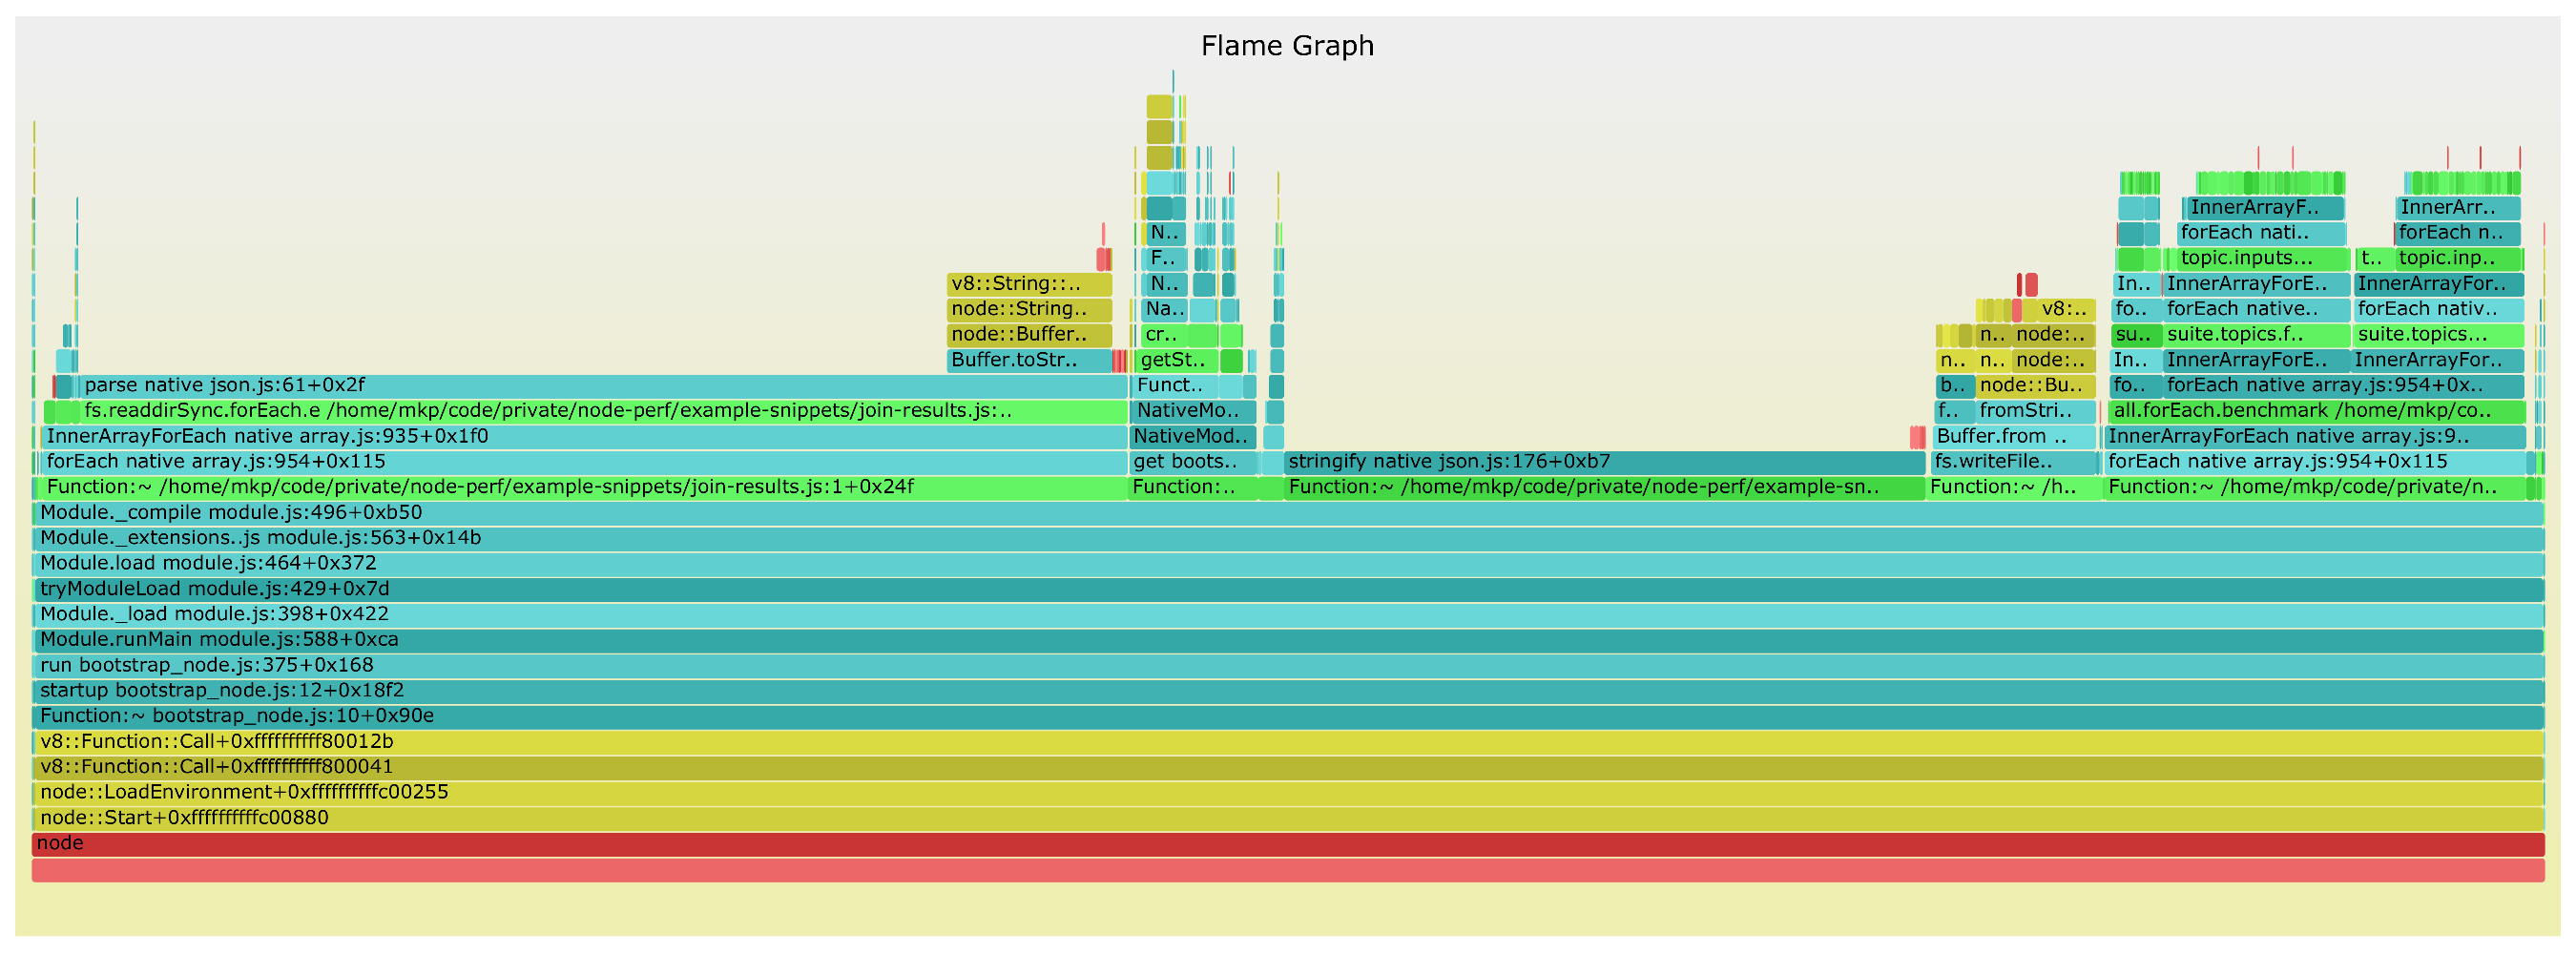
\includegraphics[width=0.8\textwidth]{pics/example-flame-graph.eps}
	\caption{Beispiel Flame-Graph eines Node.js Skripts}
	\label{fig:example-flame-graph}
\end{figure}

Beispielhaftes Code-Snippet siehe \autoref{lst:sample}.

\begin{lstlisting}[language=bash,caption={Aufnahme der \glqq real\grqq-Zeit},label={lst:sample}]
START=$(date +%s.%N)
node ${JS_FILE}
END=$(date +%s.%N)
DIFF=$(echo "$END - $START" | bc)
\end{lstlisting}

Hier kommt eine Bibliography-Referenz: \cite{booch2007object}

\lstlistoflistings

\listoffigures

\chapter*{Abkürzungen}
\markboth{Abkürzungen}{}


\begin{acronym}[Bash]
	

\acro{GC}{Garbage Collection}

\glqq Garbage Collection\grqq{} bezeichnet die automatische Speicherwaltung zur Minimierung des Speicherbedarfes eines Programmes.
\ac{GC} wird zur Laufzeit durch Identifikation von nicht mehr benötigten Speicherbereichen ausgeführt.
Im Vergleich zur manuellen Speicherverwaltung benötigt \ac{GC} mehr Ressourcen.

\end{acronym}

\bibliographystyle{alpha}
\bibliography{sources}


\chapter*{Eidesstattliche Erklärung}

Ich versichere hiermit, dass ich die von mir eingereichte Masterarbeit selbstständig verfasst, ausschließlich die angegebenen Hilfsmittel benutzt und sowohl wörtliche, als auch sinngemäße entlehnte Stellen als solche kenntlich gemacht habe. Die Arbeit hat in gleicher oder ähnlicher Form noch keiner anderen Prüfungsbehörde vorgelegen.

Brandenburg an der Havel, XX. Monat 2017

\vspace{3cm}

Vorname Nachname

\end{document}
